\documentclass[fontsize=11pt,paper=a4]{scrartcl}

\usepackage[english]{babel}
\usepackage{microtype}
\usepackage{listings}
\usepackage{hyperref}
\usepackage{csquotes}
\usepackage{graphicx}

\lstset{
  language=C,
  basicstyle=\small,
  breaklines=true
}
\frenchspacing 

%%% Maketitle metadata
\newcommand{\horrule}[1]{\rule{\linewidth}{#1}} 	

\title{
		%\vspace{-1in} 	
		\usefont{OT1}{bch}{b}{n}
		\normalfont \normalsize \textsc
		{Coursera Course: Cloud Computing} \\ [25pt]
		\horrule{0.5pt} \\[0.4cm]
		\huge Capstone Project Task 2 Report \\
		\horrule{2pt} \\[0.5cm]
}
\author{Hang Shi\\[-3pt] }
\date{\today\\[-3pt]}


\begin{document}
\maketitle

\section{Overview}
This report covers the design and implementation details for Cloud Computing Captone Project Task 2. The goals of this task are to perform the following:
\begin{itemize}
\item Extract and clean the transportation dataset, and then store the result in HDFS.
\item Answer 2 questions from Group 1, 3 questions from Group 2, and Question 3.2 using Spark. Store the results for questions from Group 2 and Question 3.2 in Cassandra.   
\end{itemize}
 
\section{Data Cleanup}
The first task is to clean and store the dataset. We  first retrieve and extract the dataset from the EBS volume snapshot by following steps in \url{http://docs.aws.amazon.com/AWSEC2/latest/UserGuide/ebs-restoring-volume.html}. One key thing to note is that we need to create EC2 instance in the same region and availabbility zone as the data EBS snapshot (snap-e1608d88 in us-east-1d).   

Afterwards, we explore the data set and decide on how we wish to clean it. Then we ignore unrelated rows and extract only the columns from the csv files. The raw data is in \path{/data/aviation/airline_ontime} directory. 

Python and Bash scripts are developed used to do the cleanup: 
\begin{itemize} 
\item A python script is developed on top of \href{https://docs.python.org/2/library/csv.html}{python CSV package} to extract the fields. 
\item Bash scripts are used to loop through all data sets. 
\end{itemize}

Such data cleanup is a one-time job. The cleaned data are stored on HDFS via below hdfs dfs command  as tab delimetered fields with each line indicating one flight. For question 3.2, only 2008 data is used. 
\begin{lstlisting}{centered}
	Cmd: hdfs dfs -copyFromLocal <local files> <hdfs dir>  
	Fields: Year, Month, Day, Weekday, FullDate, Airline, Carrier, Flight, Origin, Dest, CRSDepTime, DepDelay, ArrDelay
\end{lstlisting}

\section{System Overview}
See figure 1 for system architecture details for this project. 

\begin{figure}
\centering
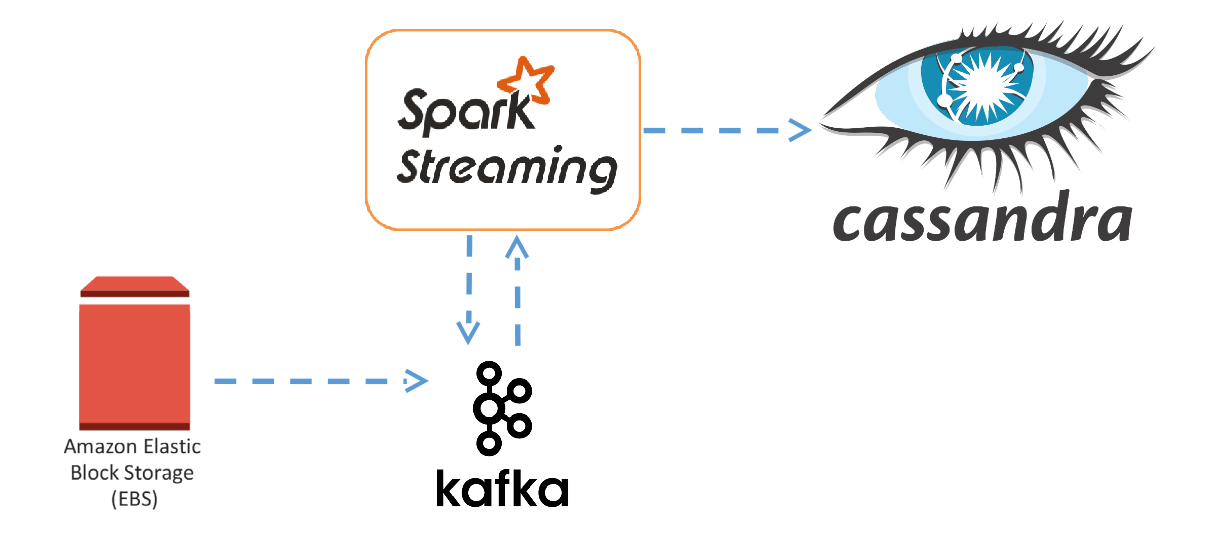
\includegraphics[width=\linewidth,,keepaspectratio]{system_architecture.png}
\caption{System Architecture for This Project.}
\label{fig:verticalcell}
\end{figure}

\subsection{Spark on EC2}
\subsection{Hadoop, Kafka, and Spark Streaming}
The system is essentially a 4 node Apache Hadoop cluster with one namenode and three datanodes running on AWS EC2. Hadoop Yarn runs and serves as the resource manager and application manager. Kafka is used to stream the cleaned data stored in HDFS to Spark, which does the RDD/Data Frame processing before storing the results to NoSQL database. 

TODO: Modify this link for EC2 Spark 

\href{https://blog.insightdatascience.com/spinning-up-a-free-hadoop-cluster-step-by-step-c406d56bae42}{Spinning Up a Free Hadoop Cluster: Step by Step}

\subsection{NOSQL Database: Cassandra} 
Cassandra cluster is deployed on the three Hadoop datanodes to provide data replication and scalability. The cluster run on the same rack and utilizes GossipingPropertyFileSnitch scheme. One of the nodes is assigned as the seed provider. Initially version 3.6 is used, but due to the support of group by is missing in 3.6, version 3.11 is used. 
 
 
\section{Group 1 Problems} 

\small \begin{itemize} 
\item Problem 1.1: Rank the top 10 most popular airports by numbers of flights to/from the airport.
\item Problem 1.2: Rank the top 10 airlines by on-time arrival performance
\end{itemize}

\textbf{Solution:} both problems are solved using same technique: stateful updates via Spark API updateStateByKey. See below for details. 
\tiny \begin{lstlisting}[language = python] 
def updateFunction(newValues, runningCount):
    return sum(newValues, runningCount or 0)
filtered = lines.map(lambda line: line.split("\t"))\
                .flatMap(lambda w: [(w[3], 1), (w[4], 1)] )\
                .reduceByKey(lambda a, b: a+b)\
                .updateStateByKey(updateFunction)\
                .transform(lambda r: r.sortBy(lambda (w, c): -c))
\end{lstlisting}

 
\section{Group 2 Problems}
\small \begin{itemize} 
\item Problem 2.1: For each airport X, rank the top-10 carriers in decreasing order of on-time departure performance from X. 
\item Problem 2.2: For each airport X, rank the top-10 airports in decreasing order of on-time departure performance from X.
\item Problem 2.3: For each source-destination pair X-Y, rank the top-10 carriers in decreasing order of on-time arrival performance at Y from X.
\item Problem 2.4: For each source-destination pair X-Y, determine the mean arrival delay (in minutes) for a flight from X to Y.
\end{itemize}

\textbf{Solution:} All four questions are solved using same approach: Spark stateful RDD transformation, Data Frame API, and Cassandra Spark API. See below two code examples: 
\tiny \begin{lstlisting}[language = python] 
# RDD Processing
def updateFunction(newValues, runningCount):
    values, counter, avg_delay = runningCount or (0., 0, 0.)
    for val in newValues: 
        values += val[0]
        counter += val[1]
    return (values, counter, values/counter) 
f1 = lines.map(lambda line:line.split(","))\
          .map(lambda f:Flight(f))\
          .map(lambda f:((f.Origin, f.Dest),(f.DepDelay, 1)))\
          .updateStateByKey(updateFunction)
filtered = f1.map(lambda (x, y):(x[0], y[2], x[1]))
filtered.foreachRDD(lambda rdd:print_rdd(rdd))
\end{lstlisting}

\tiny \begin{lstlisting}[language = python] 
# Data Frame Transformation and Data Storing 
schema = StructType([
         StructField("origin", StringType(), True),
         StructField("delay", FloatType(), True), 
         StructField("dest", StringType(), True)
         ])
df = getSqlContextInstance(rdd.context).createDataFrame(rdd, schema);  
df.show() 
#insert into cassandra 
df.write.format("org.apache.spark.sql.cassandra")\
    .mode('overwrite').options(table="g2e2", keyspace="test")\
    .save()
\end{lstlisting}






\section{Group 3 Problems}
\begin{itemize}
\item Problem 3.1. Does the popularity distribution of airports follow a Zipf distribution? If not, what distribution does it follow?
Zipf’s law stats that given some corpus or natural language utterances, the frequency of any word is inversely proportional to its rank in the frequency table. In our case it means that the airport with a higher rank should have a double number of flights compare with the next airport in rank. Even if from the Flights by Airport figure we can hope for a Zipf distribution, after doing a log-log plot we can see that Airports rank by number of flights is not following this distribution (log log for Zipf should be a straight line and is not). gnuplot tool is used to do plotting and it can be proven that this distribution is not Zipf but more a Lognormal one since the bottom half look very different than the top half. 
\item Problem 3.2. Tom wants to travel from airport X to airport Z. However, Tom also wants to stop at airport Y for some sightseeing on the way. More concretely, Tom has the following requirements (see Task 1 Queries for specific queries):
\begin{itemize}
\item A. The second leg of the journey (flight Y-Z) must depart two days after the first leg (flight X-Y). For example, if X-Y departs January 5, 2008, Y-Z must depart January 7, 2008.
\item B. Tom wants his flights scheduled to depart airport X before 12:00 PM local time and to depart airport Y after 12:00 PM local time.
\item C. Tom wants to arrive at each destination with as little delay as possible.
It is solved by creating two MapReduce Jobs. One which filter the
flights by arrival performance and the second one which computes the options Tom has and pick up the best one based on arrival performance. For the first map reduce the key is based on Origin, Destination and FlightDate. In the second MapReduce we will receive a list of best arrival flights grouped by Origin-Destination-Date and from here using the 12h departure condition we can generate for each day all the options Tom has.
\end{itemize}
\end{itemize}

\section{Optimization Techniques}
\begin{itemize}
\item Removal of unused data columns: only needed columns have been imported from the original dataset, thus lowering the needs for data transfer and storage capacity.
\item Data ordering and partitioning: the import script orders and partitions by date the data from the original dataset. This way the import process into HDFS is faster.
\item Data preload into HDFS: data  is loaded to HDFS before starting to process it. This way, we can achieve persistent storage in HDFS and fast access from HDFS.
\item During Kafka streaming, the Spark executor can't handle full speed of Kafka streaming, two approaches are used: increase the memory when inovking spark streaming, and sleep a small interval streaming between two files. 

\end{itemize} 
 
\section{Code and Video Location}
\begin{itemize}
\item Code:    \url{https://github.com/myhangshi/ccompute}
\item Video:   \url{https://vimeo.com/241272936}
\end{itemize} 
 

\end{document}
